% 2008 年江苏卷第 22 题：棱长 1 的正方体，P 在对角线 BD1 上。
% 来源 PDF：gaokaomath-src/普通高考/2008/2008江苏.pdf
% SHA-256：b998b93963143559a1ce800a6d320de618883b0e22ee5130b7666a2374caeba0
% 原页：2008江苏.pdf 第 2 页（A3 三栏）第 3 栏，书页码 458。
% 绘制依据：按原页斜投影：上底 A1B1C1D1、下底 ABCD，P 在 BD1 上；
%   被遮挡的棱 A1D1、D1C1、DD1 与 BD1、AP、CP 用虚线。
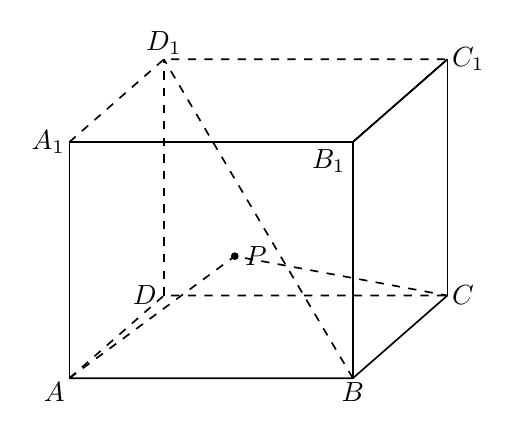
\begin{tikzpicture}[scale=1.0, semithick, every node/.style={inner sep=1.4pt}]
  \coordinate (A) at (0.00,0.00);
  \coordinate (B) at (3.60,0.00);
  \coordinate (C) at (4.80,1.05);
  \coordinate (D) at (1.20,1.05);
  \coordinate (A1) at (0.00,3.00);
  \coordinate (B1) at (3.60,3.00);
  \coordinate (C1) at (4.80,4.05);
  \coordinate (D1) at (1.20,4.05);
  \coordinate (P) at (2.10,1.55);

  \draw (A) -- (B) -- (C);
  \draw (A) -- (A1);
  \draw (B) -- (B1);
  \draw (C) -- (C1);
  \draw (A1) -- (B1) -- (C1);
  \draw (B1) -- (C1);

  \draw[dashed] (A) -- (D) -- (C);
  \draw[dashed] (D) -- (D1);
  \draw[dashed] (A1) -- (D1) -- (C1);
  \draw[dashed] (B) -- (D1);
  \draw[dashed] (A) -- (P) -- (C);

  \fill (P) circle (1.4pt);

  \node[below left] at (A) {$A$};
  \node[below] at (B) {$B$};
  \node[right] at (C) {$C$};
  \node[left=1pt] at (D) {$D$};
  \node[left] at (A1) {$A_1$};
  \node[below left=1pt] at (B1) {$B_1$};
  \node[right] at (C1) {$C_1$};
  \node[above] at (D1) {$D_1$};
  \node[right=2pt] at (P) {$P$};
\end{tikzpicture}
